% !TeX root = ../../main.tex
% Add the above to each chapter to make compiling the PDF easier in some editors.

\chapter{Experiments and Results}\label{chapter:experiments}

This chapter presents the experiments performed in different selected environments. The selected algorithms with their configurations are discussed. We then conclude with the experimental results and discuss the goal and aim of the experiment.

\section{Distributed Experiments}

This section shows the conducted experiments starting from non-distributed based experiments until having a high-performance scalable algorithm and the multi-agent environment in the experiments. We start from the base experiment and compare the output results with each experiment.

% !TeX root = ../../main.tex

\subsection{2-DOF Arm Gym Base Non-Distributed Experiment}

This experiment is the \textit{base experiment} of a set of experiments for reinforcement learning in robots simulations. In this way, we perform an initial experiment with a selected reinforcement learning algorithm on the 2-DOF robotic arm to achieve the goal of the environment and reach the target as quickly and efficiently as possible. Based on this experiment, we plan to build on it more advanced experiments to show the effect of using distribution for reinforcement learning tasks and the benefit of parallelizing the environments to enhance the performance of the agents and solve the task quickly. Performing the experiment, we plan to extend it to a more complex environment with modified reward function and on different physics engine to compare the existing reinforcement learning platforms and express the difference in comparison. Hence, we study the effect of distribution and transferability between the different engine and the efficiency between them.

\subsubsection{Aim of the experiment}

This experiment is designed to be performed on non-distributed setup using only the power of CPUs, which make it the base experiment for the performed experiments and to be able to compare between different selected reinforcement learning methods and algorithms and show the effect of using distributed algorithms and parallelizing experiment's environment to achieve the efficiency and speed wanted to perform reinforcement learning experiments. 

We want to investigate how the agent will perform in the experiment, the time taken to run the experiment, the average episode reward the agent will get and whether the agent will be able to solve the environment in constrained stopping conditions.

\subsubsection{Setup and configurations}

In this section we describe the setup of the experiment and how it was performed. Firstly, we introduce and describe the RoboReacher robotics arm environment provided by OpenAI Gym and PyBullet physics simulator. Then, based on the environment description, we present the observation space, action space and reward function of the experiment as a base towards the learning process and achieving environment goal. Subsequently, we describe the learning process. For this, we present the reinforcement learning algorithm and neural network architecture used.


\subsubsection{Environment Description: 2-DOF Robot Arm | Roboschool Reacher}
Roboschool is an open-source software for robot simulation, integrated with OpenAI Gym. The selected environment is \textit{Reacher Environment}~\ref{fig:openai_reacher}: A robotic arm consist of two linked joints places in a squared arena surrounding it along with a moving sphere (target). The goal of the robotics arm it to reach target sphere and maintain following the point until the end of the episode. 

\begin{figure}[!htb]
		\centering
		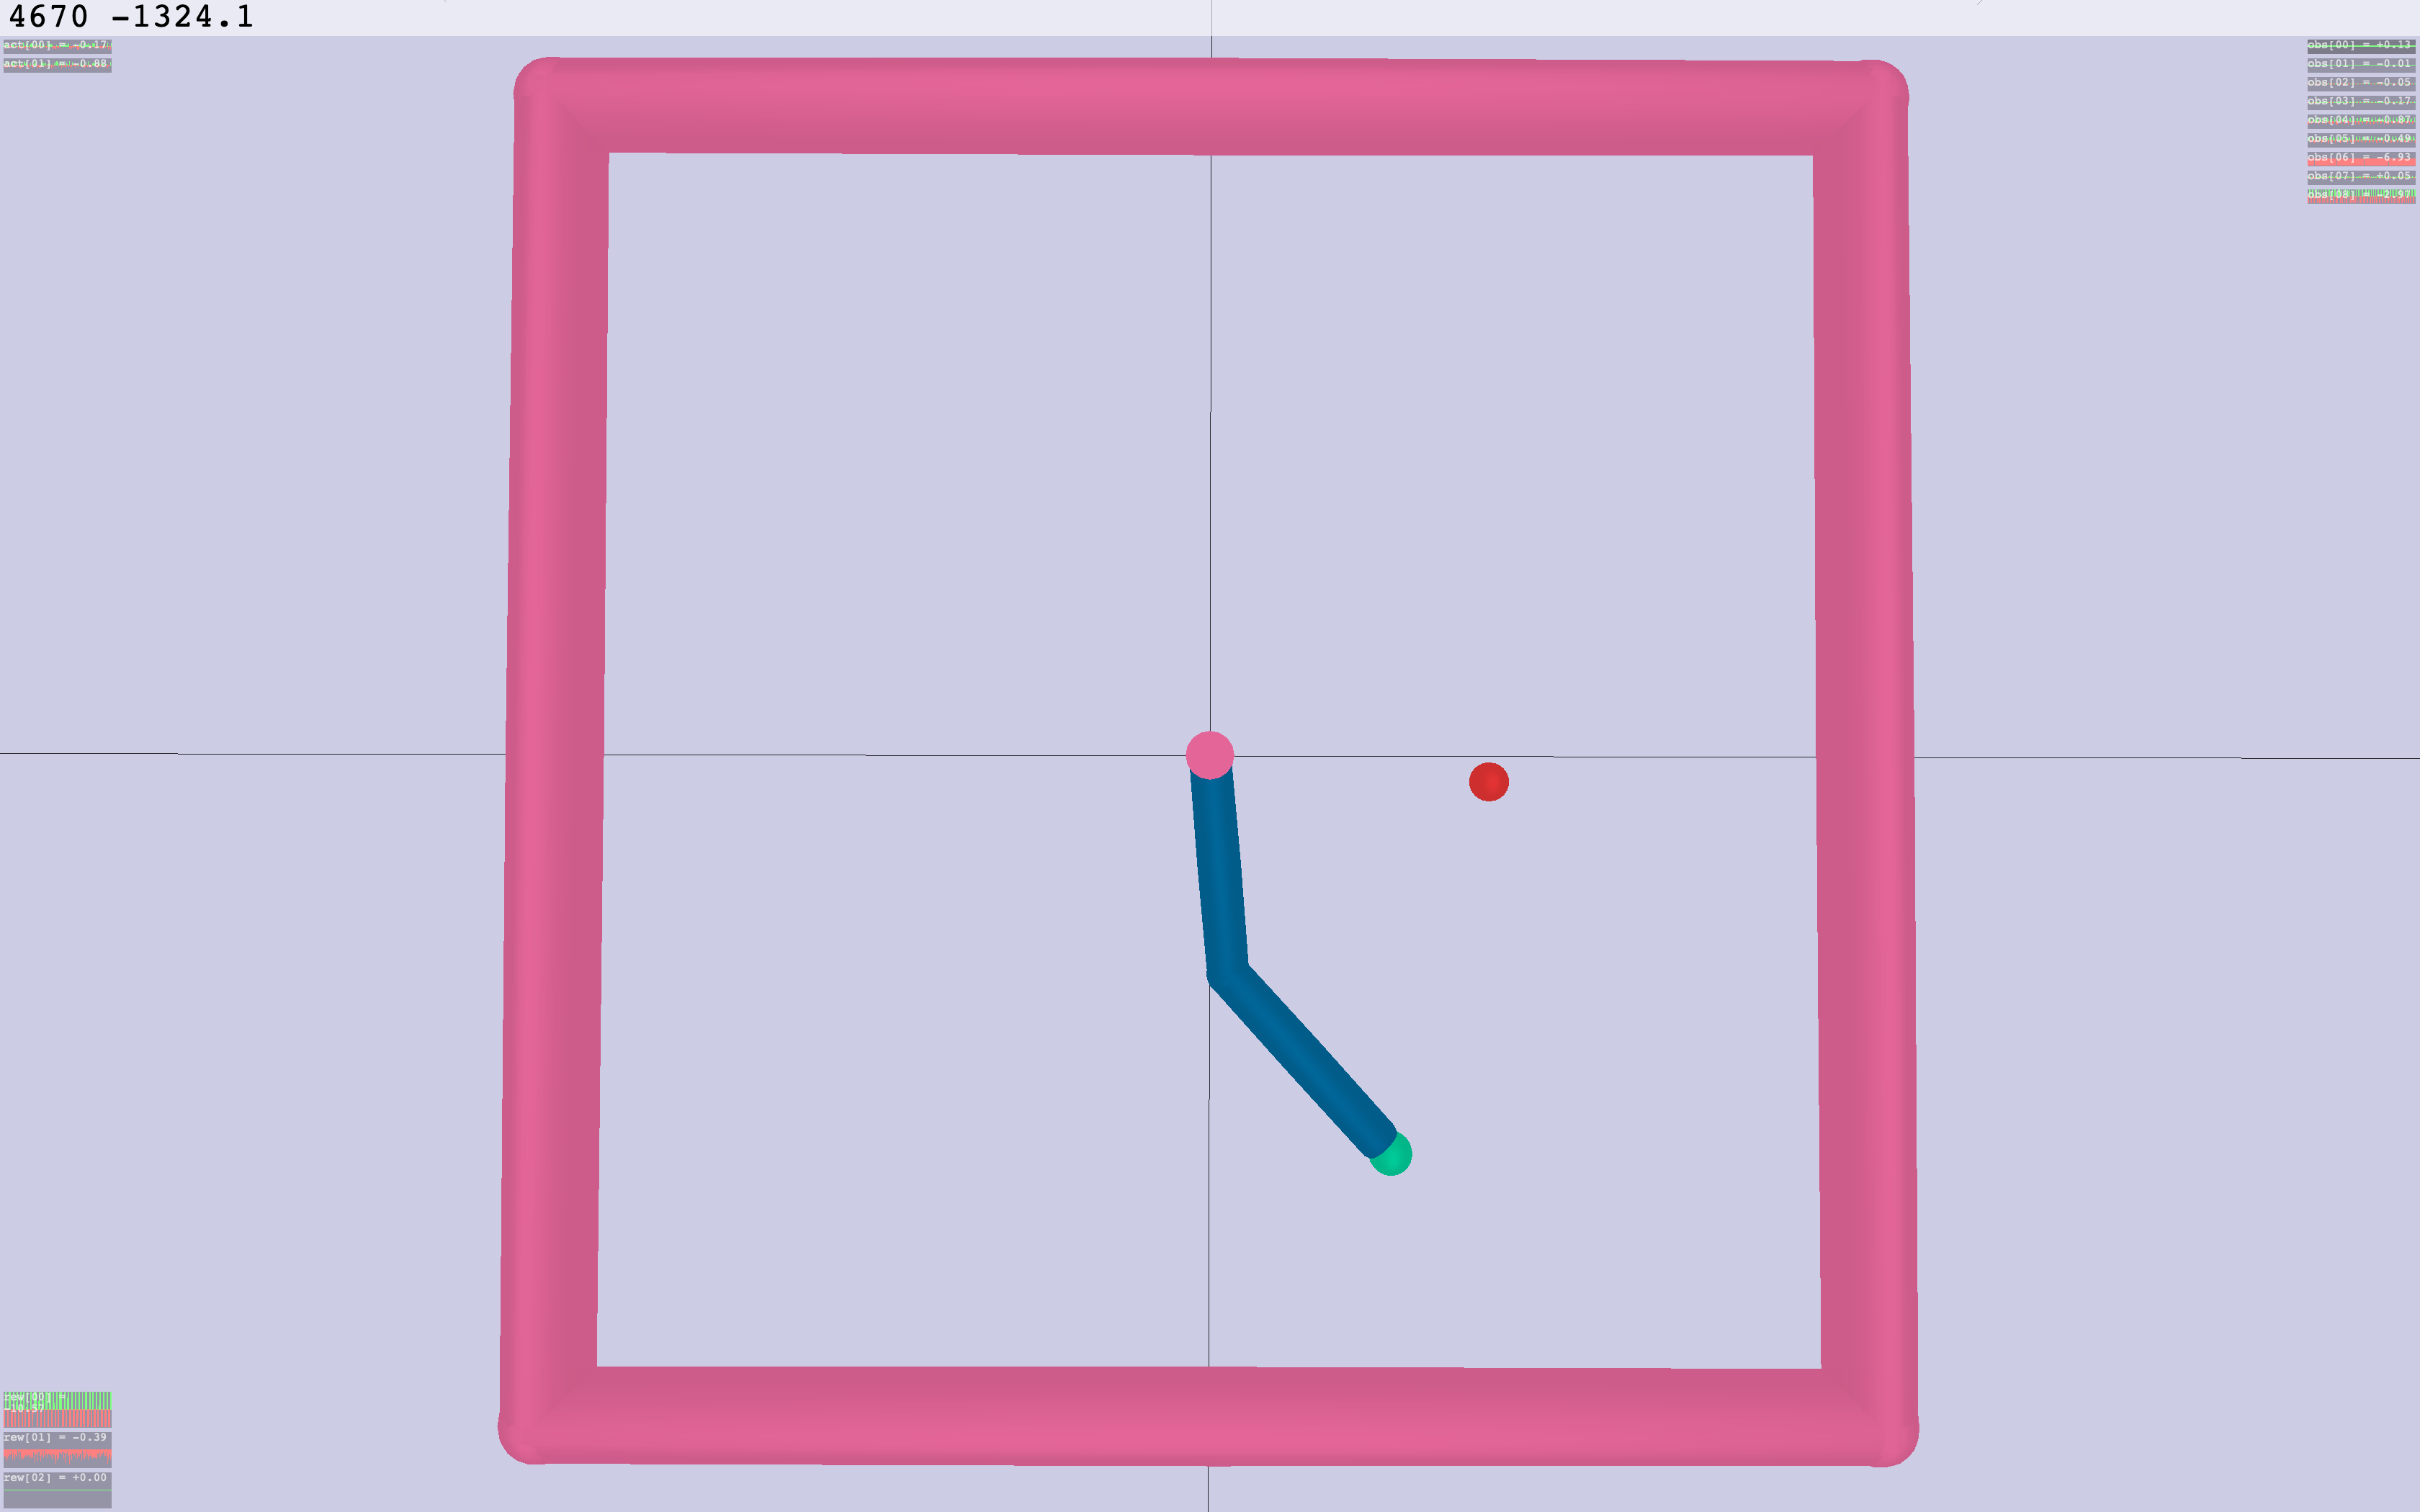
\includegraphics[width=0.7\linewidth]{figures/envs/openai_roboreacher.png}
		\caption{OpenAI Reacher Environment}
		\label{fig:openai_reacher}
\end{figure}

\subsubsection{Observation Space}

The observation space of the environment, shown in the table~\ref{tab:gym_reacher_obs} below, consist of \textbf{9 variables} corresponding to the position of the target sphere, the x-axis and y-axis components of the vector from the target to the fingertip, cos(theta) and sin(theta) for the joints and the angular velocity of the fingertip in the x and y directions.

\begin{table}[!htb]
		\centering
		\begin{tabular}{|c|c|}
				\hline
				\multicolumn{2}{|c|}{{\ul \textit{\textbf{Observation Space}}}}                                                                                   \\ \hline
				\multirow{2}{*}{\textbf{Target Position}}                                                                      & \textit{X Position}              \\ \cline{2-2} 
																																																								& \textit{Y Position}              \\ \hline
				\multirow{2}{*}{\textbf{Arm to Target Vector}}                                                                 & \textit{Position vector 0}       \\ \cline{2-2} 
																																																								& \textit{Position vector 1}       \\ \hline
				\multirow{2}{*}{\textbf{\begin{tabular}[c]{@{}c@{}}Current Relative Position\\ of Central Joint\end{tabular}}} & \textit{cosine of central joint} \\ \cline{2-2} 
						& \textit{sine of central joint}   \\ \hline
				\multirow{2}{*}{\textbf{\begin{tabular}[c]{@{}c@{}}Current Relative Position\\ of Elbow Joint\end{tabular}}}   & \textit{cosine of elbow joint}   \\ \cline{2-2} 
						& \textit{sine of elbow joint}     \\ \hline
		\end{tabular}
		\caption{Gym Reacher Observation Information}
		\label{tab:gym_reacher_obs}
\end{table}

\subsubsection{Action Space}

The action space of the environment, shown in the table~\ref{tab:gym_reacher_actions} below, is a continuous one which indicated the torque applied on both of the robotic arm joints.

\begin{table}[!htb]
		\centering
		\begin{tabular}{|c|c|}
				\hline
				\multicolumn{2}{|c|}{{\ul \textit{\textbf{Action Space (Continuous)}}}}                             \\ \hline
				\multirow{2}{*}{\textbf{Center Joint Torque}} & \multirow{2}{*}{\textit{range(-1, 1)}} \\
																												&                                        \\ \hline
				\multirow{2}{*}{\textbf{Elbow Joint Torque}}  & \multirow{2}{*}{\textit{range(-1, 1)}} \\
																												&                                        \\ \hline
		\end{tabular}
				\caption{Gym Reacher Action Information}
				\label{tab:gym_reacher_actions}
\end{table}

\subsubsection{Reward Function}

\let\realurl\url
\renewcommand{\url}[1]{%
  \realurl{#1}%
  \wlog{URLX #1 }%
}

The reward function\footnote{\url{https://github.com/openai/roboschool/blob/master/roboschool/gym_reacher.py\#L70}} is designed based on the distance between the arm and the target along with electricity cost of the torque and angular velocity of the arm with small epsilon amount in case of the joint is stuck. 


\subsubsection{Algorithm}

In this experiment, \textbf{Proximal Policy Optimization (PPO)} algorithm is selected to be the base algorithm for our initial experiment. 

Below are the default configuration for PPO algorithm:
\lstinputlisting[language=Python]{chapters/04/ppo_default.py}

followed by this experiment setup and configuration as listed below:
\begin{table}[!htb]
		\centering
		\begin{tabular}{|c|l|l|c|l|l|}
				\hline
				\multicolumn{6}{|c|}{\textit{\textbf{Gym Reacher PPO 1st Experiment: Non-Distributed Experiment}}}                                                        \\ \hline
				\multicolumn{3}{|c|}{\textbf{env}}                                  & \multicolumn{3}{c|}{RoboschoolReacher-v1}                                           \\ \hline
				\multicolumn{3}{|c|}{\textbf{env\_type}}                            & \multicolumn{3}{c|}{OpenAI Environment}                                             \\ \hline
				\multicolumn{3}{|c|}{\textbf{run: Algorithms}}                      & \multicolumn{3}{c|}{\cellcolor[HTML]{C0C0C0}\textbf{PPO}}                           \\ \hline
				\multicolumn{3}{|c|}{}                                              & \multicolumn{3}{c|}{\cellcolor[HTML]{E1F7E1}episode\_reward\_mean = 21}             \\ \cline{4-6} 
				\multicolumn{3}{|c|}{\multirow{-2}{*}{\textbf{stop condition}}}     & \multicolumn{3}{c|}{\cellcolor[HTML]{E1F7E1}time-steps\_total = 10000000: 10M Steps} \\ \hline
				\multicolumn{3}{|c|}{\textbf{gamma}}                                & \multicolumn{3}{c|}{0.99}                                                           \\ \hline
				\multicolumn{3}{|c|}{\textbf{kl coefficient}}                            & \multicolumn{3}{c|}{1.0}                                                            \\ \hline
				\multicolumn{3}{|c|}{\textbf{num\_sgd\_iter}}                       & \multicolumn{3}{c|}{20}                                                             \\ \hline
				\multicolumn{3}{|c|}{\textbf{lr}}                                   & \multicolumn{3}{c|}{0.0001}                                                         \\ \hline
				\multicolumn{3}{|c|}{\textbf{sgd\_minibatch\_size}}                 & \multicolumn{3}{c|}{1000}                                                           \\ \hline
				\multicolumn{3}{|c|}{\textbf{train\_batch\_size}}                   & \multicolumn{3}{c|}{25000}                                                          \\ \hline
				\multicolumn{3}{|c|}{\textbf{batch\_mode}}                          & \multicolumn{3}{c|}{complete\_episodes}                                             \\ \hline
				\multicolumn{3}{|c|}{\textbf{observation\_filter}}                  & \multicolumn{3}{c|}{MeanStdFilter}                                                  \\ \hline
				\multicolumn{3}{|c|}{\cellcolor[HTML]{C0C0C0}\textbf{num\_gpus}}    & \multicolumn{3}{c|}{\cellcolor[HTML]{C0C0C0}0}                                      \\ \hline
				\multicolumn{3}{|c|}{\cellcolor[HTML]{C0C0C0}\textbf{num\_workers}} & \multicolumn{3}{c|}{\cellcolor[HTML]{C0C0C0}0}                                      \\ \hline
		\end{tabular}
		\caption{Gym Reacher PPO 1st Experiment: Non-Distributed Experiment}
		\label{tab:gym_reacher_ppo_1st_exp}
\end{table}


\subsubsection{Neural Network Architecture}
In this simple environment, the observation space is not a visual (pixel raw images) observation, which means it won't require a convolutional neural network to process it, Hence, the algorithm will be using fully connected neural network consist of input layer of 9 variables for the observation, two hidden layers with 256 neuron for each layer, and the output layer of 2 neurons corresponding to the actions send to the environment as shown below~\ref{fig:ppo_nn}:

\begin{figure}[!htb]
		\centering
		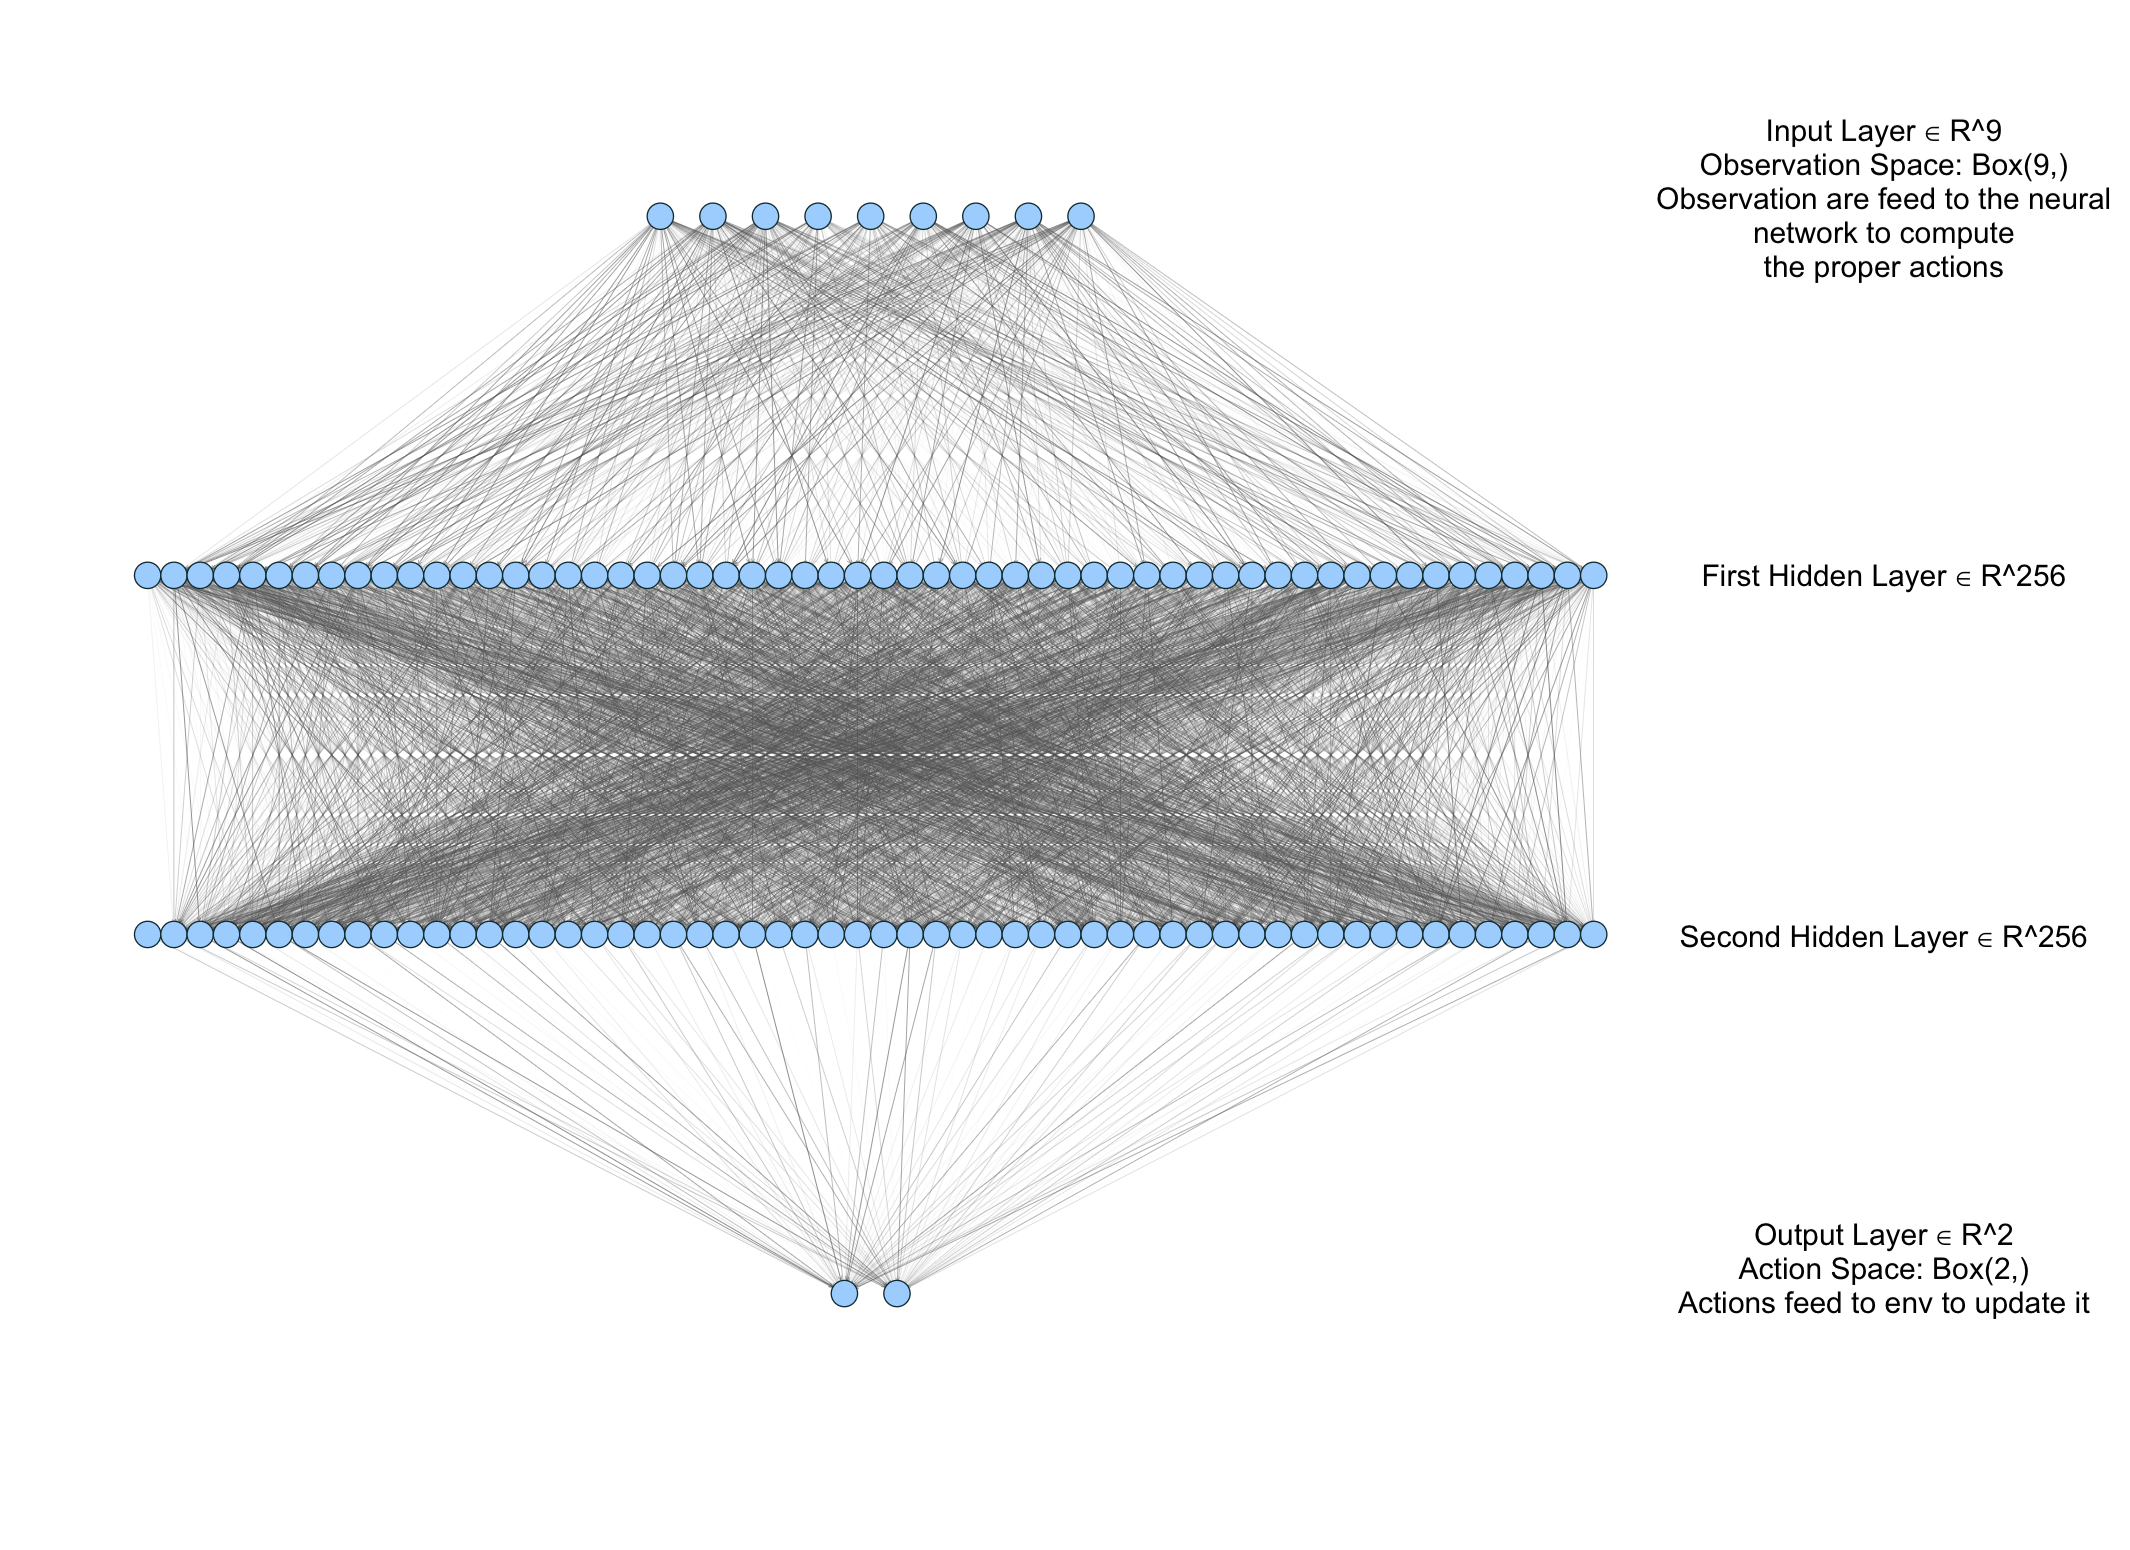
\includegraphics[width=\linewidth]{figures/exps/1st_exp/ppo_nn}
		\caption{PPO Neural Network Architecture}
		\label{fig:ppo_nn}
\end{figure}


\subsubsection{Experiment Results}

After performing the experiment with a stopping conditions either \textit{\textbf{reaching an average reward of 21 or total time steps of the agent is 10M steps}} as indicated in ~\ref{tab:gym_reacher_ppo_1st_exp}. We measure the environment and training process to evaluate the experiment and be able to compare with others.

We start by measuring the maximum reward~\ref{fig:1st_exp_max_eps_reward} the agent could get from the environment, as shown in the figure below, the maximum the agent could obtain is 30 reward over all the training time-steps it has performed.
\begin{figure}[!htb]
	\centering
	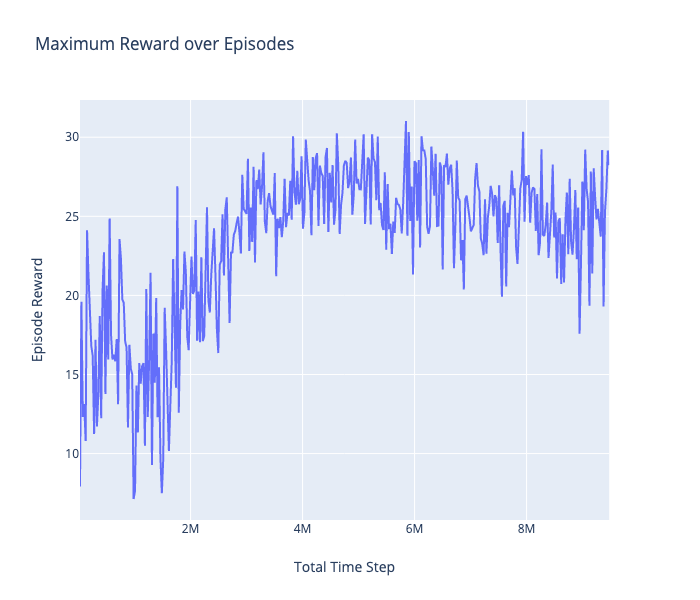
\includegraphics[width=\linewidth]{figures/exps/1st_exp/max_eps_reward}
	\caption{Maximum Reward over Episodes}
	\label{fig:1st_exp_max_eps_reward}
\end{figure}

Followed by measuring what is the minimum reward the agent is getting, shown in the figure~\ref{fig:1st_exp_min_eps_reward}, and the observation shows that the agent is stuck under -30 reward and it's performance has high variance before completing 2M time-steps.
\begin{figure}[H]
	\centering
	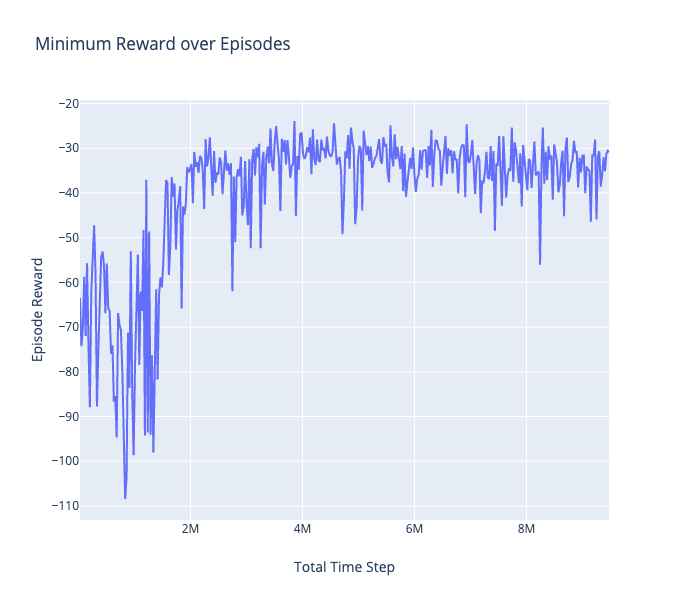
\includegraphics[width=\linewidth]{figures/exps/1st_exp/min_eps_reward}
	\caption{Minimum Reward over Episodes}
	\label{fig:1st_exp_min_eps_reward}
\end{figure}
The experiment was constrained under the conditions of reaching average reward of 21 or completing 10M steps. Based on the following figure~\ref{fig:1st_exp_avg_eps_reward}, the agent was not able to obtain the required reward for the first stopping condition. Hence, the agent completed the 10M time-steps without achieving the goal of the environment. This indicated the bad performance for this agent (getting only +1 reward) and the training process in a non-distributed environment wasn't sufficient to complete the required task.
\begin{figure}[H]
	\centering
	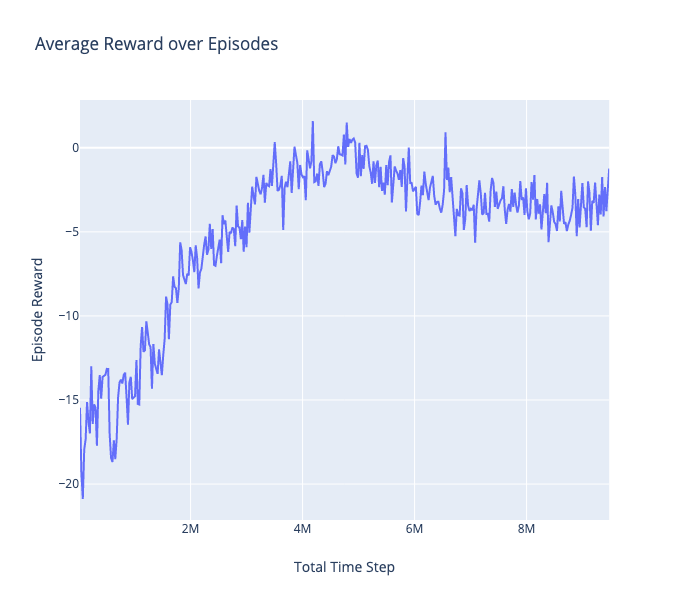
\includegraphics[width=\linewidth]{figures/exps/1st_exp/avg_eps_reward}
	\caption{Average Reward over Episodes}
	\label{fig:1st_exp_avg_eps_reward}
\end{figure}
The following measurement~\ref{fig:1st_exp_total_loss} describe the total loss of the algorithm which shows high variance and indicate that the algorithm needed more time to reduce the loss and reach a minimum better than this to enhance the agent performance.
\begin{figure}[H]
	\centering
	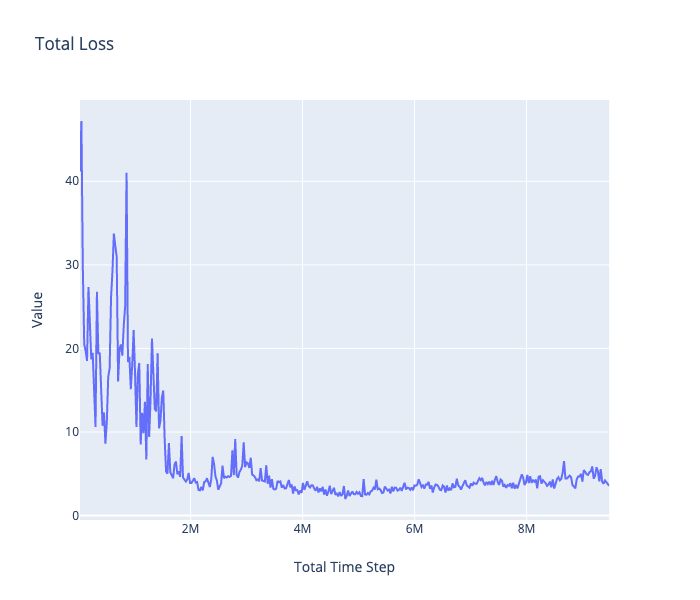
\includegraphics[width=\linewidth]{figures/exps/1st_exp/total_loss}
	\caption{Total Loss}
	\label{fig:1st_exp_total_loss}
\end{figure}
The most important metric for the experiment, which is the aim we want to reduce as much as possible, is the \textbf{total training time} for the experiment. The following figure shows the training time for the experiment in hours. This indicated how much time needed to perform such an experiment. From the figure~\ref{fig:1st_exp_total_training_time}, the experiment time is approximately \textbf{4 Hours}, which is very huge for performing normal task in a simple robotic environment.
\begin{figure}[H]
	\centering
	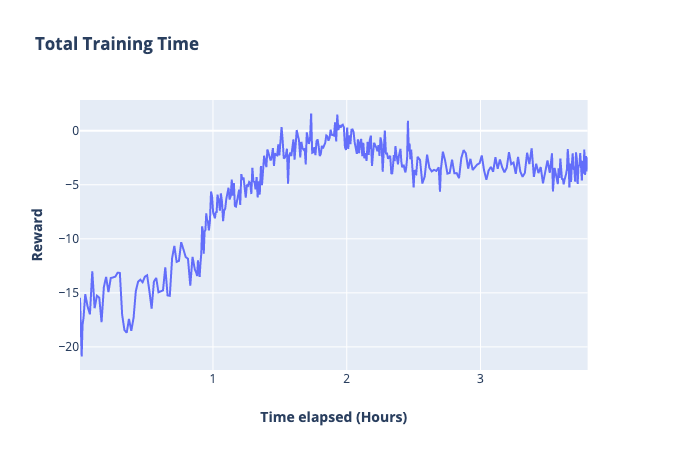
\includegraphics[width=\linewidth]{figures/exps/1st_exp/total_time}
	\caption{Total Training Time}
	\label{fig:1st_exp_total_training_time}
\end{figure}

\subsubsection{Conclusion}

In this experiment, we perform a training and evaluation for the simple robotic task using ppo algorithm in non-distributed setup to train our agent. we conclude that the experiment took a large amount of time to train the agent (4 hours) and at the end the agent didn't solve the required task and the learning process was not successful. 

Summary for the results:
\begin{itemize}
	\item The agent completed the 10M steps.
	\item The agent could not solve the required task.
	\item The average the agent could get did not exceed 1 reward over the whole episodes~\ref{fig:1st_exp_avg_eps_reward}.
	\item The maximum the agent could get did not exceed 30 reward over the whole episodes~\ref{fig:1st_exp_max_eps_reward}.
	\item The performance of the agent is not quite good.
	\item The total loss is not improving and didn't reach global minimum~\ref{fig:1st_exp_total_loss}.
	\item The total time elapsed exceed 3.5 hours for such a simple environment and task~\ref{fig:1st_exp_total_training_time}.
\end{itemize}
\clearpage

% !TeX root = ../../main.tex

\subsection{2-DOF Arm Distributed Experiment}

This experiment is identical to the first experiment we have conducted except that the version of the PPO algorithm is now distributed among multiple workers and the experiment is using GPU power in addition to CPU. In this way, the experiment can be compared with the non-distributed version to spot the performance between them and compare the output, reward received and the total time for executing the experiments. 

\subsubsection{Aim of the experiment}

This experiment is designed to be performed on distributed setup using the power of GPUs and CPUs. The selected algorithm is identical with the same configuration as the previous one, the only difference is the number of workers and the usage of the GPU. In this way, the experiment can be compared with the base experiment to spot the differences between both setups and show the effect on the performance for both the agent and the running time.

The experiment is also conducted to investigate how the agent will perform in the experiment, the time taken to run the experiment, the average episode reward the agent will get and whether the agent will be able to solve the environment in constrained stopping conditions.

\subsubsection{Setup and configurations}

The experiment setup and configuration are the same as the previous experiment, except we have \textbf{a number of workers are 11 workers and using one GPU}.

\subsubsection{Experiment Results}

The experiment is performed until an average reward of 21 achieved or for a maximum of 10000000 (10M) steps if no improvement is observable. For evaluating the model performance, we compare the average reward between both experiments. In total, we measure the following metrics averaging over each episode:
\begin{itemize}
		\item The Maximum reward the agent can achieve
		\item The Average reward the agent can achieve
		\item The Minimum reward the agent can achieve
		\item The Total Time Steps obtained by the agent
		\item The Total loss for the selected algorithm
		\item The Total Time taken to perform the experiment
\end{itemize}

Starting from the maximum reward the agent has obtained, we observe that the agent could quickly learn how to reach the target sphere after only 1M time-steps, passing the non-distributed agent score. After 4M time-steps, the agent achieves the maximum reward (40) that can be obtained in the environment. In the following figure~\ref{fig:2nd_exp_max_eps_reward}, the performance of both the agent for the maximum reward in the environment is shown below:
\begin{figure}[!htb]
		\centering
		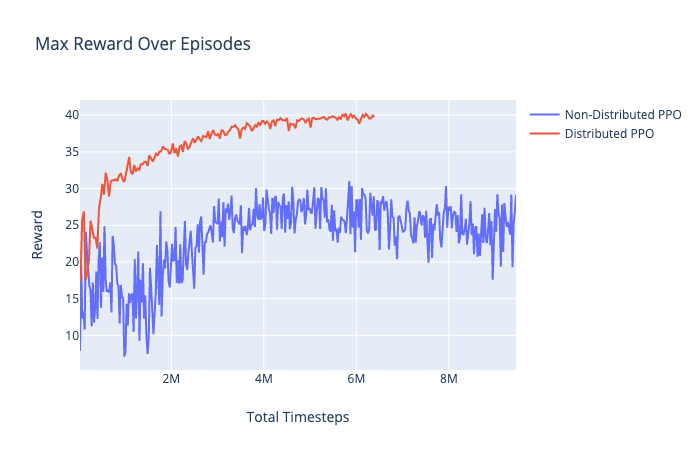
\includegraphics[width=\linewidth]{figures/exps/2nd_exp/max_eps_reward.png}
		\caption{Maximum Reward over Episodes}
		\label{fig:2nd_exp_max_eps_reward}
\end{figure}

Since the experiments are constrained under the conditions of reaching an average reward of 21 or completing 10M steps, we compare the performance of both agents for the average reward. The observation is the distributed version of the agent exceeds the average reward obtained by the non-distributed agent after only 500,000 time-steps. Followed by performance improvement over time-steps as the agent reach 15 rewards after 2M time-steps, and reaching 20 rewards after 4M time-steps, leading the agent to solve the environment and achieve the specified 21 average reward after 6M time-steps only. Hence, the agent performance is better than the previous one and could solve the environment effectively before reaching 10M time-steps. The following figure~\ref{fig:2nd_exp_avg_eps_reward}, illustrate the performance of each agent for obtaining the average rewards.
\begin{figure}[!htb]
		\centering
		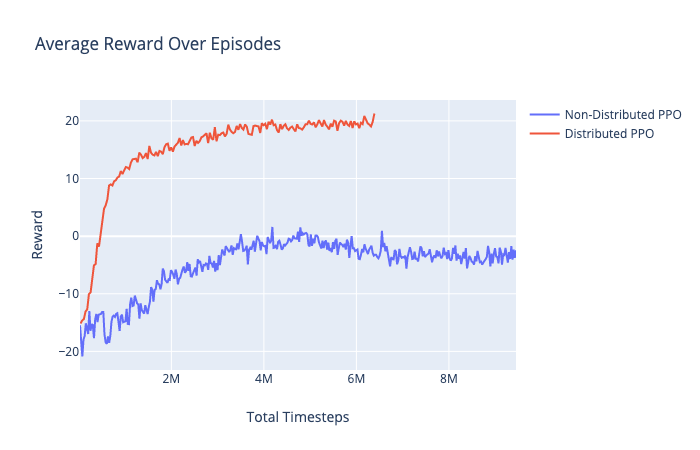
\includegraphics[width=\linewidth]{figures/exps/2nd_exp/avg_eps_reward.png}
		\caption{Maximum Reward over Episodes}
		\label{fig:2nd_exp_avg_eps_reward}
\end{figure}

Comparing the losses of both experiments, we observe the huge decrease and stability of the Distributed PPO total loss after 500,000 time-steps and reaching approximately 0 after 2M time-steps. In contrast with the non-distributed PPO, which shows a high variance in the total loss between 7 and 3 values and never reaching zero as shown in the following figure~\ref{fig:2nd_exp_total_loss}
\begin{figure}[!htb]
		\centering
		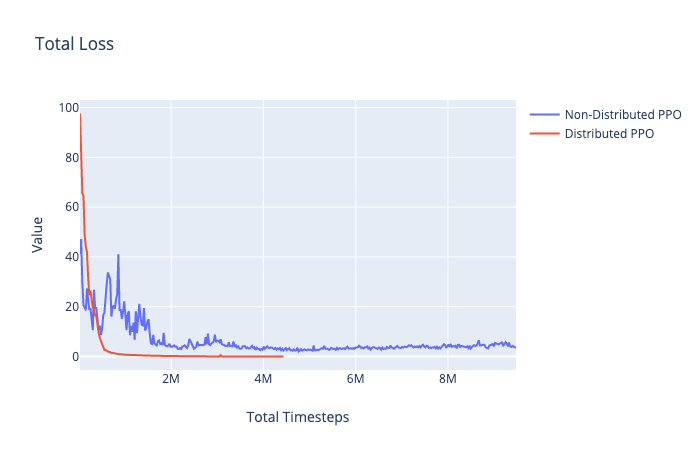
\includegraphics[width=\linewidth]{figures/exps/2nd_exp/total_loss.png}
		\caption{Total Loss}
		\label{fig:2nd_exp_total_loss}
\end{figure}

Comparing between the experiment's total taken time is crucial as it's one of the main key concept for our experiments. Running the two experiments multiple times with different seeds, we observe that the distributed experiment take half the time needed to perform the non-distributed experiment, making it much faster to train and execute reinforcement learning algorithms in distributed setup. The following figure~\ref{fig:2nd_exp_total_training_time} show the time taken for each experiment per hour.
\begin{figure}[!htb]
		\centering
		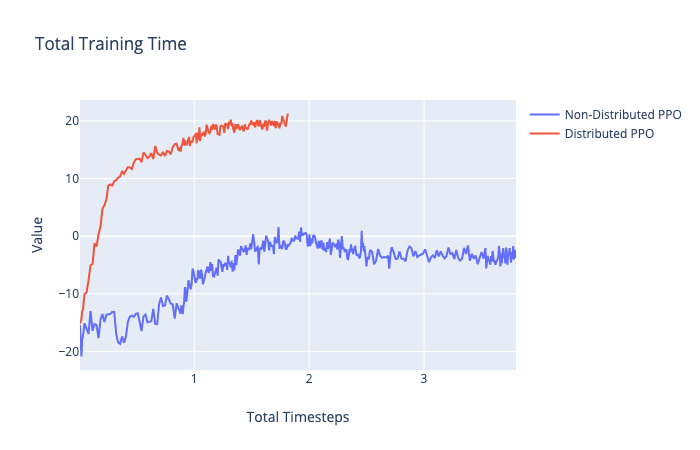
\includegraphics[width=\linewidth]{figures/exps/2nd_exp/total_training_time.png}
		\caption{Total Training Time}
		\label{fig:2nd_exp_total_training_time}
\end{figure}


\subsubsection{Conclusion}

In this experiment, we perform a training and evaluation for the robotic arm using distributed version of the PPO algorithm to train our agent. As shown in the results, we conclude that the distributed experiment is much better than the non-distributed version in the training time, the learning process for the agent and for solving the required task.

Summary for the results:
\begin{itemize}
	\item The agent solved the required task.
	\item The agent only required 6M time-steps to complete the task.
	\item The average the agent gets 21.2 reward over the whole episodes (figure~\ref{fig:2nd_exp_avg_eps_reward}).
	\item The maximum the agent could get exceed 40.5 reward over the whole episodes (figure~\ref{fig:2nd_exp_max_eps_reward}).
	\item The performance of the agent better than the first one.
	\item The total time elapsed did not exceed 2 hours (figure~\ref{fig:2nd_exp_total_training_time}).
\end{itemize}
\clearpage

% !TeX root = ../../main.tex

\subsection{2-DOF Arm Multi-Agent Distributed Experiment}

Since the distributed setup achieves higher performance, we will be moving to a more higher and complex distributed algorithms which provide high-performance throughput and can scale to support multi-agent environments and simulate in a larger scale for achieving faster training and performance in the least amount of time providing high-performance computing power.

\subsubsection{Aim of the experiment}

This experiment is designed to be performed on large multi-agents scale in a distributed setup using APE-X DDPG Algorithm for continuous spaces. Using a single GPU learner and many CPU workers for experience collection. Experience collection can scale to hundreds of CPU workers due to the distributed prioritization of experience prior to storage in replay buffers.

We want to investigate how the agent will perform in the experiment, the time taken to run the experiment, the average episode reward the agent will get and whether the agent will be able to solve the environment in constrained stopping conditions.

\subsubsection{Setup and configurations}

In this experiment, the Distributed Prioritized Experience Replay (Ape-X) algorithm is selected to train the agents in the experiments. Since this experiment is Scalable Multi-Agent, the experiment was performed with multiple numbers of agents and environment per each agent to test the Scalability and efficiency and determine the best setup for the experiment.

Below is the default configuration for the Ape-X algorithm:
\lstinputlisting[language=Python]{chapters/04/apex_default.py}

followed by this experiment setup and configuration as listed below:
\begin{table}[!htb]
	\centering
	\begin{tabular}{|c|l|l|c|l|l|}
		\hline
		\multicolumn{6}{|c|}{\textit{\textbf{Gym Reacher Ape-X 3rd Experiment: Multi-Agent Distributed Experiment}}}                                                        \\ \hline
		\multicolumn{3}{|c|}{\textbf{env}}                                            & \multicolumn{3}{c|}{RoboschoolReacher-v1}                                            \\ \hline
		\multicolumn{3}{|c|}{\textbf{env\_type}}                                      & \multicolumn{3}{c|}{OpenAI Environment}                                              \\ \hline
		\multicolumn{3}{|c|}{\textbf{run: Algorithms}}                                & \multicolumn{3}{c|}{\cellcolor[HTML]{C0C0C0}\textbf{APEX\_DDPG}}                     \\ \hline
		\multicolumn{3}{|c|}{}                                                        & \multicolumn{3}{c|}{\cellcolor[HTML]{E1F7E1}episode\_reward\_mean = 21}              \\ \cline{4-6} 
		\multicolumn{3}{|c|}{\multirow{-2}{*}{\textbf{stop condition}}}               & \multicolumn{3}{c|}{\cellcolor[HTML]{E1F7E1}time-steps\_total = 10000000: 10M Steps} \\ \hline
		\multicolumn{3}{|c|}{\textbf{use\_huber}}                                     & \multicolumn{3}{c|}{True}                                                            \\ \hline
		\multicolumn{3}{|c|}{\textbf{clip\_rewards}}                                  & \multicolumn{3}{c|}{False}                                                           \\ \hline
		\multicolumn{3}{|c|}{\textbf{n\_step}}                                        & \multicolumn{3}{c|}{3}                                                               \\ \hline
		\multicolumn{3}{|c|}{\textbf{exploration\_ou\_noise\_scale}}                  & \multicolumn{3}{c|}{1.0}                                                             \\ \hline
		\multicolumn{3}{|c|}{\textbf{target\_network\_update\_freq}}                  & \multicolumn{3}{c|}{50000}                                                           \\ \hline
		\multicolumn{3}{|c|}{\textbf{tau}}                                            & \multicolumn{3}{c|}{1.0}                                                             \\ \hline
		\multicolumn{3}{|c|}{\textbf{evaluation\_interval}}                           & \multicolumn{3}{c|}{5}                                                               \\ \hline
		\multicolumn{3}{|c|}{\textbf{evaluation\_num\_episodes}}                      & \multicolumn{3}{c|}{MeanStdFilter}                                                   \\ \hline
		\multicolumn{3}{|c|}{\cellcolor[HTML]{C0C0C0}\textbf{num\_gpus}}              & \multicolumn{3}{c|}{\cellcolor[HTML]{C0C0C0}1}                                       \\ \hline
		\multicolumn{3}{|c|}{\cellcolor[HTML]{C0C0C0}\textbf{num\_workers}}           & \multicolumn{3}{c|}{\cellcolor[HTML]{C0C0C0}11}                                      \\ \hline
		\multicolumn{3}{|c|}{\cellcolor[HTML]{C0C0C0}\textbf{num\_envs\_per\_worker}} & \multicolumn{3}{c|}{\cellcolor[HTML]{C0C0C0}grid\_search: [32, 16]}                  \\ \hline
	\end{tabular}
	\caption{Gym Reacher Ape-X 3rd Experiment: Multi-Agent Distributed Experiment}
	\label{tab:gym_reacher_apex_3rd_exp}
\end{table}

As shown in the configuration table~\ref{tab:gym_reacher_apex_3rd_exp} above, we setup the number of environments to be for the first time \textbf{32 per each worker} leading the experiment to have \textbf{384 parallel environment} running in the experiment. The second run of the experiment have \textbf{16 environment per worker}, in this way the experiment have \textbf{192 environment} running in the experiment. The number of the environment can be much bigger that this in there are more powerful computing provided.


\subsubsection{Experiment Results}

The experiment is performed until an average reward of 21 achieved or for a maximum of 10000000 (10M) steps if no improvement is observable. For evaluating the model performance, we compare the average reward between both experiments. In total, we measure the following metrics averaging over each episode:
\begin{itemize}
	\item The Maximum reward the agent can achieve
	\item The Average reward the agent can achieve
	\item The Total Time Steps obtained by the agent
	\item The Total Time taken to perform the experiment
\end{itemize}

Starting from the maximum reward the agent has obtained, the agent could quickly learn and surpass both distributed and non-distributed PPO algorithm after only 2M time-steps. Achieve (+40.4) the maximum reward in the environment. In the following figure~\ref{fig:3rd_exp_max_eps_reward}, the performance of all the agents for the maximum reward in the environment is shown below:
\begin{figure}[!htb]
	\centering
	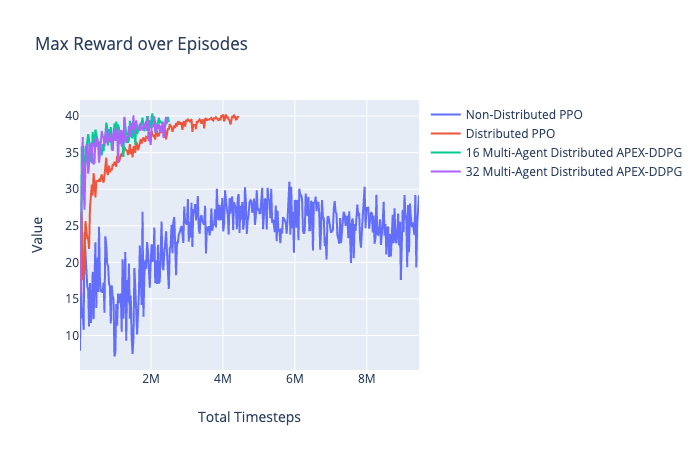
\includegraphics[width=\linewidth]{figures/exps/3rd_exp/max_eps_reward.png}
	\caption{Maximum Reward over Episodes}
	\label{fig:3rd_exp_max_eps_reward}
\end{figure}

Comparing the performance of the three agents for the average reward. The observation are the distributed apex-ddpg version exceed (+10) average reward after only 100,000 time-steps. Followed by performance improvement over time-steps as the agent reach 21 reward after 2M time-steps, leading the agent to solve the environment and achieve the specified 21 average reward before completing 3M time-steps. Hence, the agent performance is better than the two previous agents and could solve the environment effectively before reaching 3M time-steps. The following figure~\ref{fig:3rd_exp_avg_eps_reward}, illustrate the performance of each agent for obtaining the average rewards.
\begin{figure}[!htb]
	\centering
	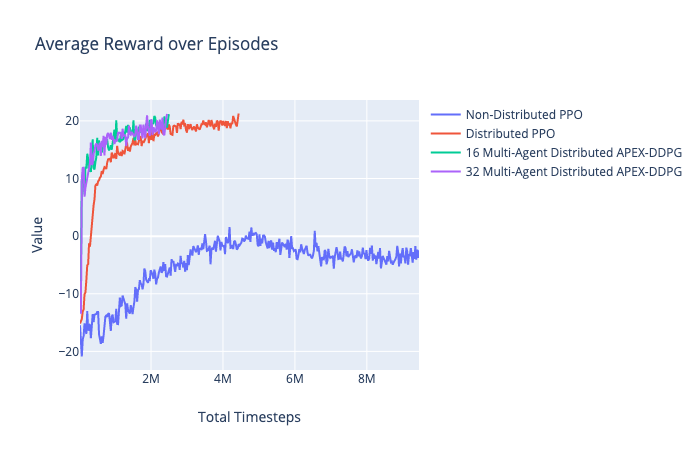
\includegraphics[width=\linewidth]{figures/exps/3rd_exp/avg_eps_reward.png}
	\caption{Maximum Reward over Episodes}
	\label{fig:3rd_exp_avg_eps_reward}
\end{figure}

The experiment's total taken time is the best factor in this experiment as the algorithm with the huge number of parallel environment was able to finish the task under only (1 Hour) of training. Exceeding the time for both the experiments and utilizing the use of GPU and parallel environment to achieve the goal quickly. Hence, using powerful high-throughput algorithms leads to much faster training time. The following figure~\ref{fig:3rd_exp_total_training_time} show the time taken for each experiment per hour.
\begin{figure}[!htb]
	\centering
	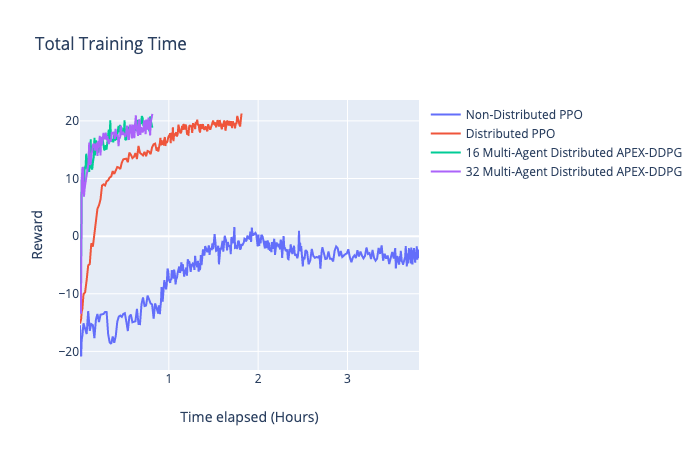
\includegraphics[width=\linewidth]{figures/exps/3rd_exp/total_training_time.png}
	\caption{Total Training Time}
	\label{fig:3rd_exp_total_training_time}
\end{figure}


\subsubsection{Conclusion}

In this experiment, we perform a training and evaluation for the robotic arm using distributed APEX-DDPG algorithm to train our agent. As shown in the results, we conclude that using high-throughput powerful algorithm in a distributed setup leads to have the best outcome for both completing a task and reducing the total time of the experiment.

Summary for the results:
\begin{itemize}
	\item The agent solved the required task.
	\item The agent only required 2.2M time-steps to complete the task.
	\item The average the agent gets 21.5 reward over the whole episodes (figure~\ref{fig:3rd_exp_avg_eps_reward}).
	\item The maximum the agent could get exceed 40.3 reward over the whole episodes (figure~\ref{fig:3rd_exp_max_eps_reward}).
	\item The performance of the agent better than the previous agents.
	\item The total time elapsed did not exceed 1 hours (~47 minutes) (figure~\ref{fig:3rd_exp_total_training_time}).
\end{itemize}
\clearpage

\section{Transferability Between Physics Engines}

This section shows an experimental approach on how to transfer pre-trained agent from one environment to another different environment using different physics engine. Followed by transferring knowledge learned in 2D space into 3D space and how the agent will behave in the new environment.

% !TeX root = ../../main.tex

\subsection{Transferring from Gym to Unity 2-DOF Base Environment}

In this experiment, we create a similar environment in Unity to test the transferability between different two physics engine. This experiment is conducted to test the trained agent on a new different environment which has the same observation and action spaces like the environment that was used for training with a different reward function. In this way, we will be using the trained agent from the third experiment to test it on this experiment and observe the performance and behaviour of the agent.

\subsubsection{Setup and configurations}

In this section we describe the setup of the experiment and how it was performed. Firstly, we introduce and describe the RoboReacher robotics arm environment provided by OpenAI Gym and PyBullet physics simulator. Then, based on the environment description, we present the observation space, action space and reward function of the experiment as a base towards the learning process and achieving environment goal. Subsequently, we describe the learning process. For this, we present the reinforcement learning algorithm and neural network architecture used.


\subsubsection{Environment Description}
Using Unity physics engine and Unity ML-Agent, we have built a new 2-DOF robotic environment, shown in the figure below~\ref{fig:unity_reacher}, which is similar to OpenAI Gym environment. The environment has the same observation and action spaces like gym environment and we have modified the reward function to be more complex in this environment to test the behavior of the trained agent.

\begin{figure}[!htb]
		\centering
				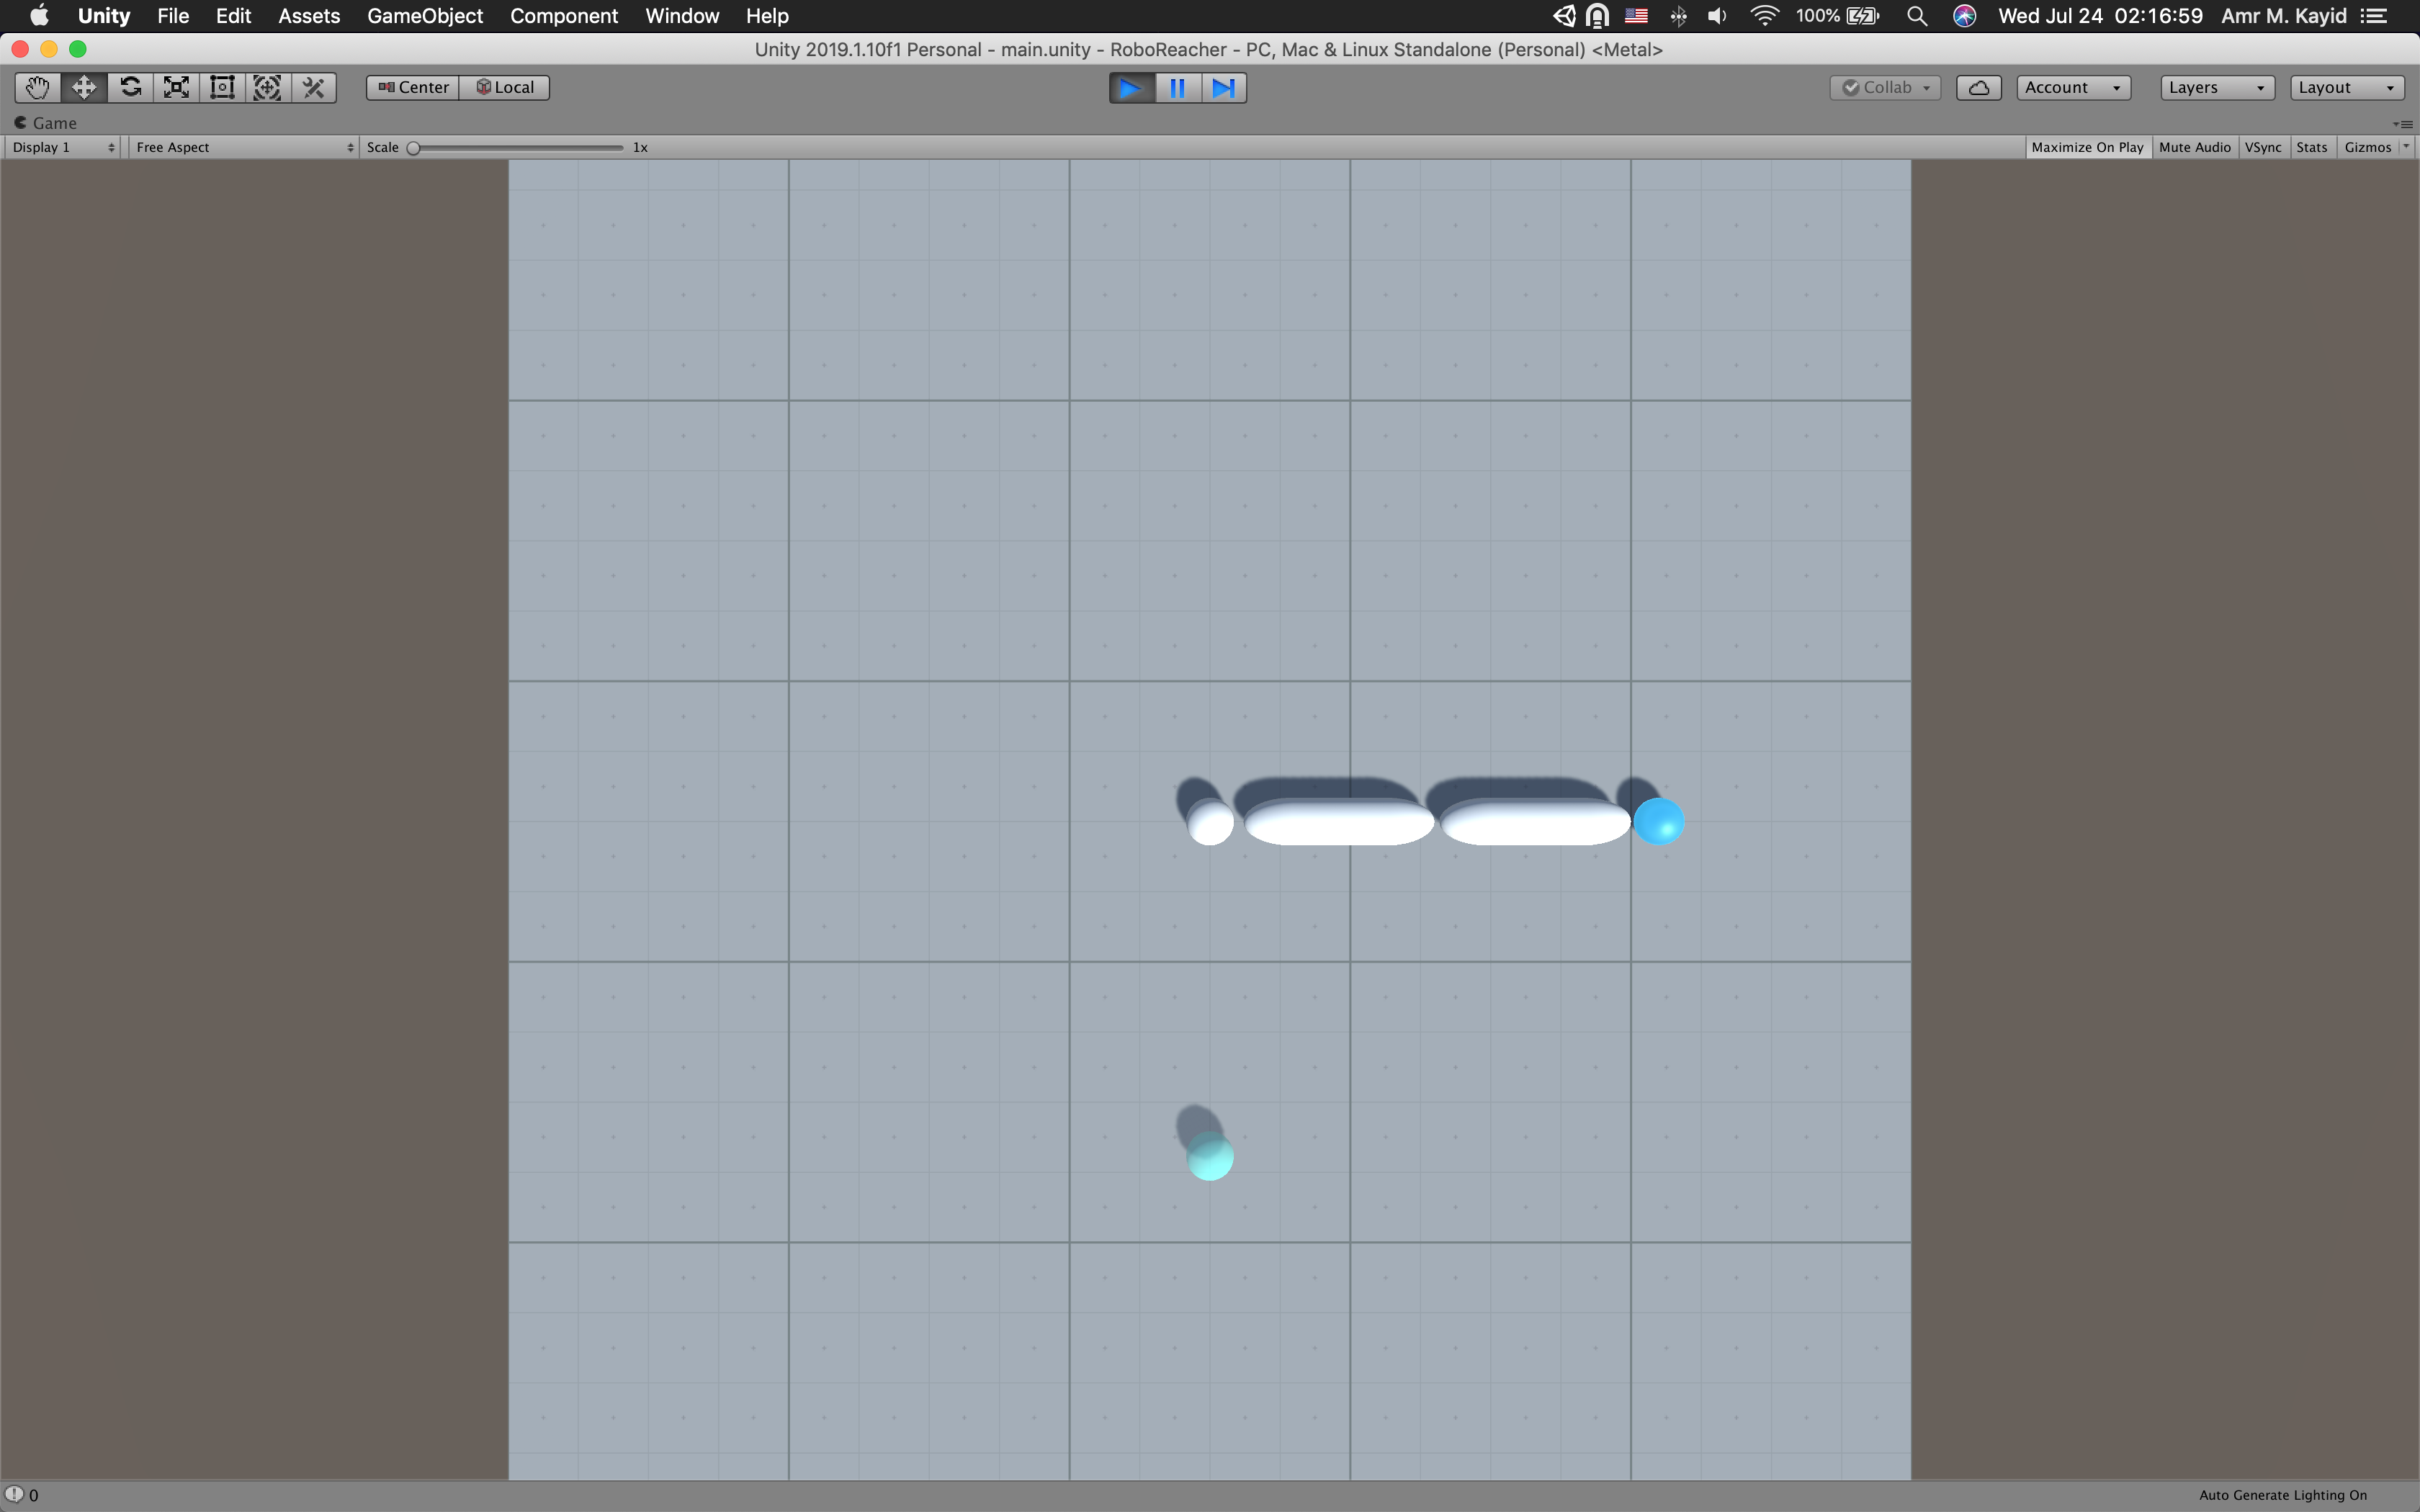
\includegraphics[width=0.7\linewidth]{figures/envs/unity_roboreacher.png}
				\caption{Unity 2-DOF Environment}
				\label{fig:unity_reacher}
\end{figure}

\subsubsection{Reward Function}

The reward function for this environment is different as we modify it to only give a reward of (+0.1) for the agent if the agent can reach the target sphere and keep moving with it along a circular path. Hence, the reward function is described as \textbf{\(R(\tau)=+0.1\)}.

\subsubsection{Experiment Results}

Since this is an evaluation experiment where we have the trained agent from the 3rd experiment, the evaluation will be based on the average reward the agent can obtain after running for 1M time-steps. In this experiment, the agent was able to obtain an average reward ranging from 15 to 20 over the whole testing time-steps as shown in the figure below~\ref{fig:unity2d_avg_reward}.

\begin{figure}[!htb]
		\centering
		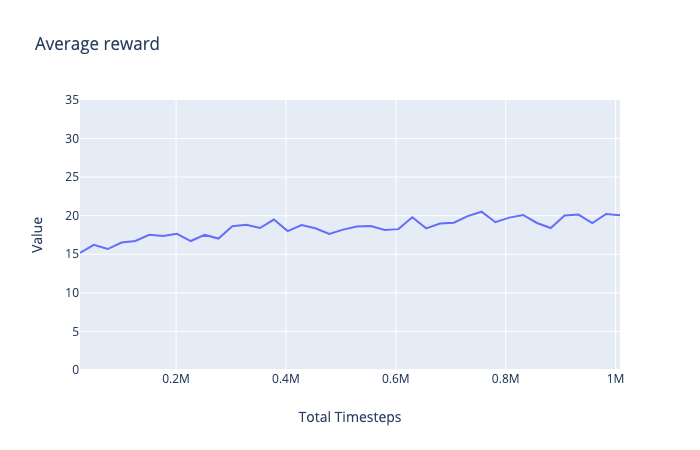
\includegraphics[width=0.7\linewidth]{figures/exps/unity2d.png}
		\caption{Unity 2-DOF Average Reward}
		\label{fig:unity2d_avg_reward}
\end{figure}


\subsubsection{Conclusion}

In this experiment, we were able to transfer learning a pre-trained agent from openai gym environment to a new similar designed unity environment which has a slightly different reward function. We conclude that the agent was able to follow the sphere while it is moving and obtain an average reward of 20. Hence transferring trained agent to new engine was successful.
\clearpage

% !TeX root = ../../main.tex

\subsection{Transferring from Gym to Unity 2-DOF Base Environment}

In this experiment, we create a similar environment in Unity to test the transferability between different two physics engine. This experiment is conducted to test the trained agent on a new different environment which has the same observation and action spaces like the environment that was used for training with a different reward function. In this way, we will be using the trained agent from the third experiment to test it on this experiment and observe the performance and behaviour of the agent.

\subsubsection{Setup and configurations}

In this section we describe the setup of the experiment and how it was performed. Firstly, we introduce and describe the RoboReacher robotics arm environment provided by OpenAI Gym and PyBullet physics simulator. Then, based on the environment description, we present the observation space, action space and reward function of the experiment as a base towards the learning process and achieving environment goal. Subsequently, we describe the learning process. For this, we present the reinforcement learning algorithm and neural network architecture used.


\subsubsection{Environment Description}
Using Unity physics engine and Unity ML-Agent, we have built a new 2-DOF robotic environment~\ref{fig:unity_reacher} which is similar to OpenAI Gym environment. The environment has the same observation and action spaces like gym environment and we have modified the reward function to be more complex in this environment to test the behavior of the trained agent.

\begin{figure}[!htb]
		\centering
				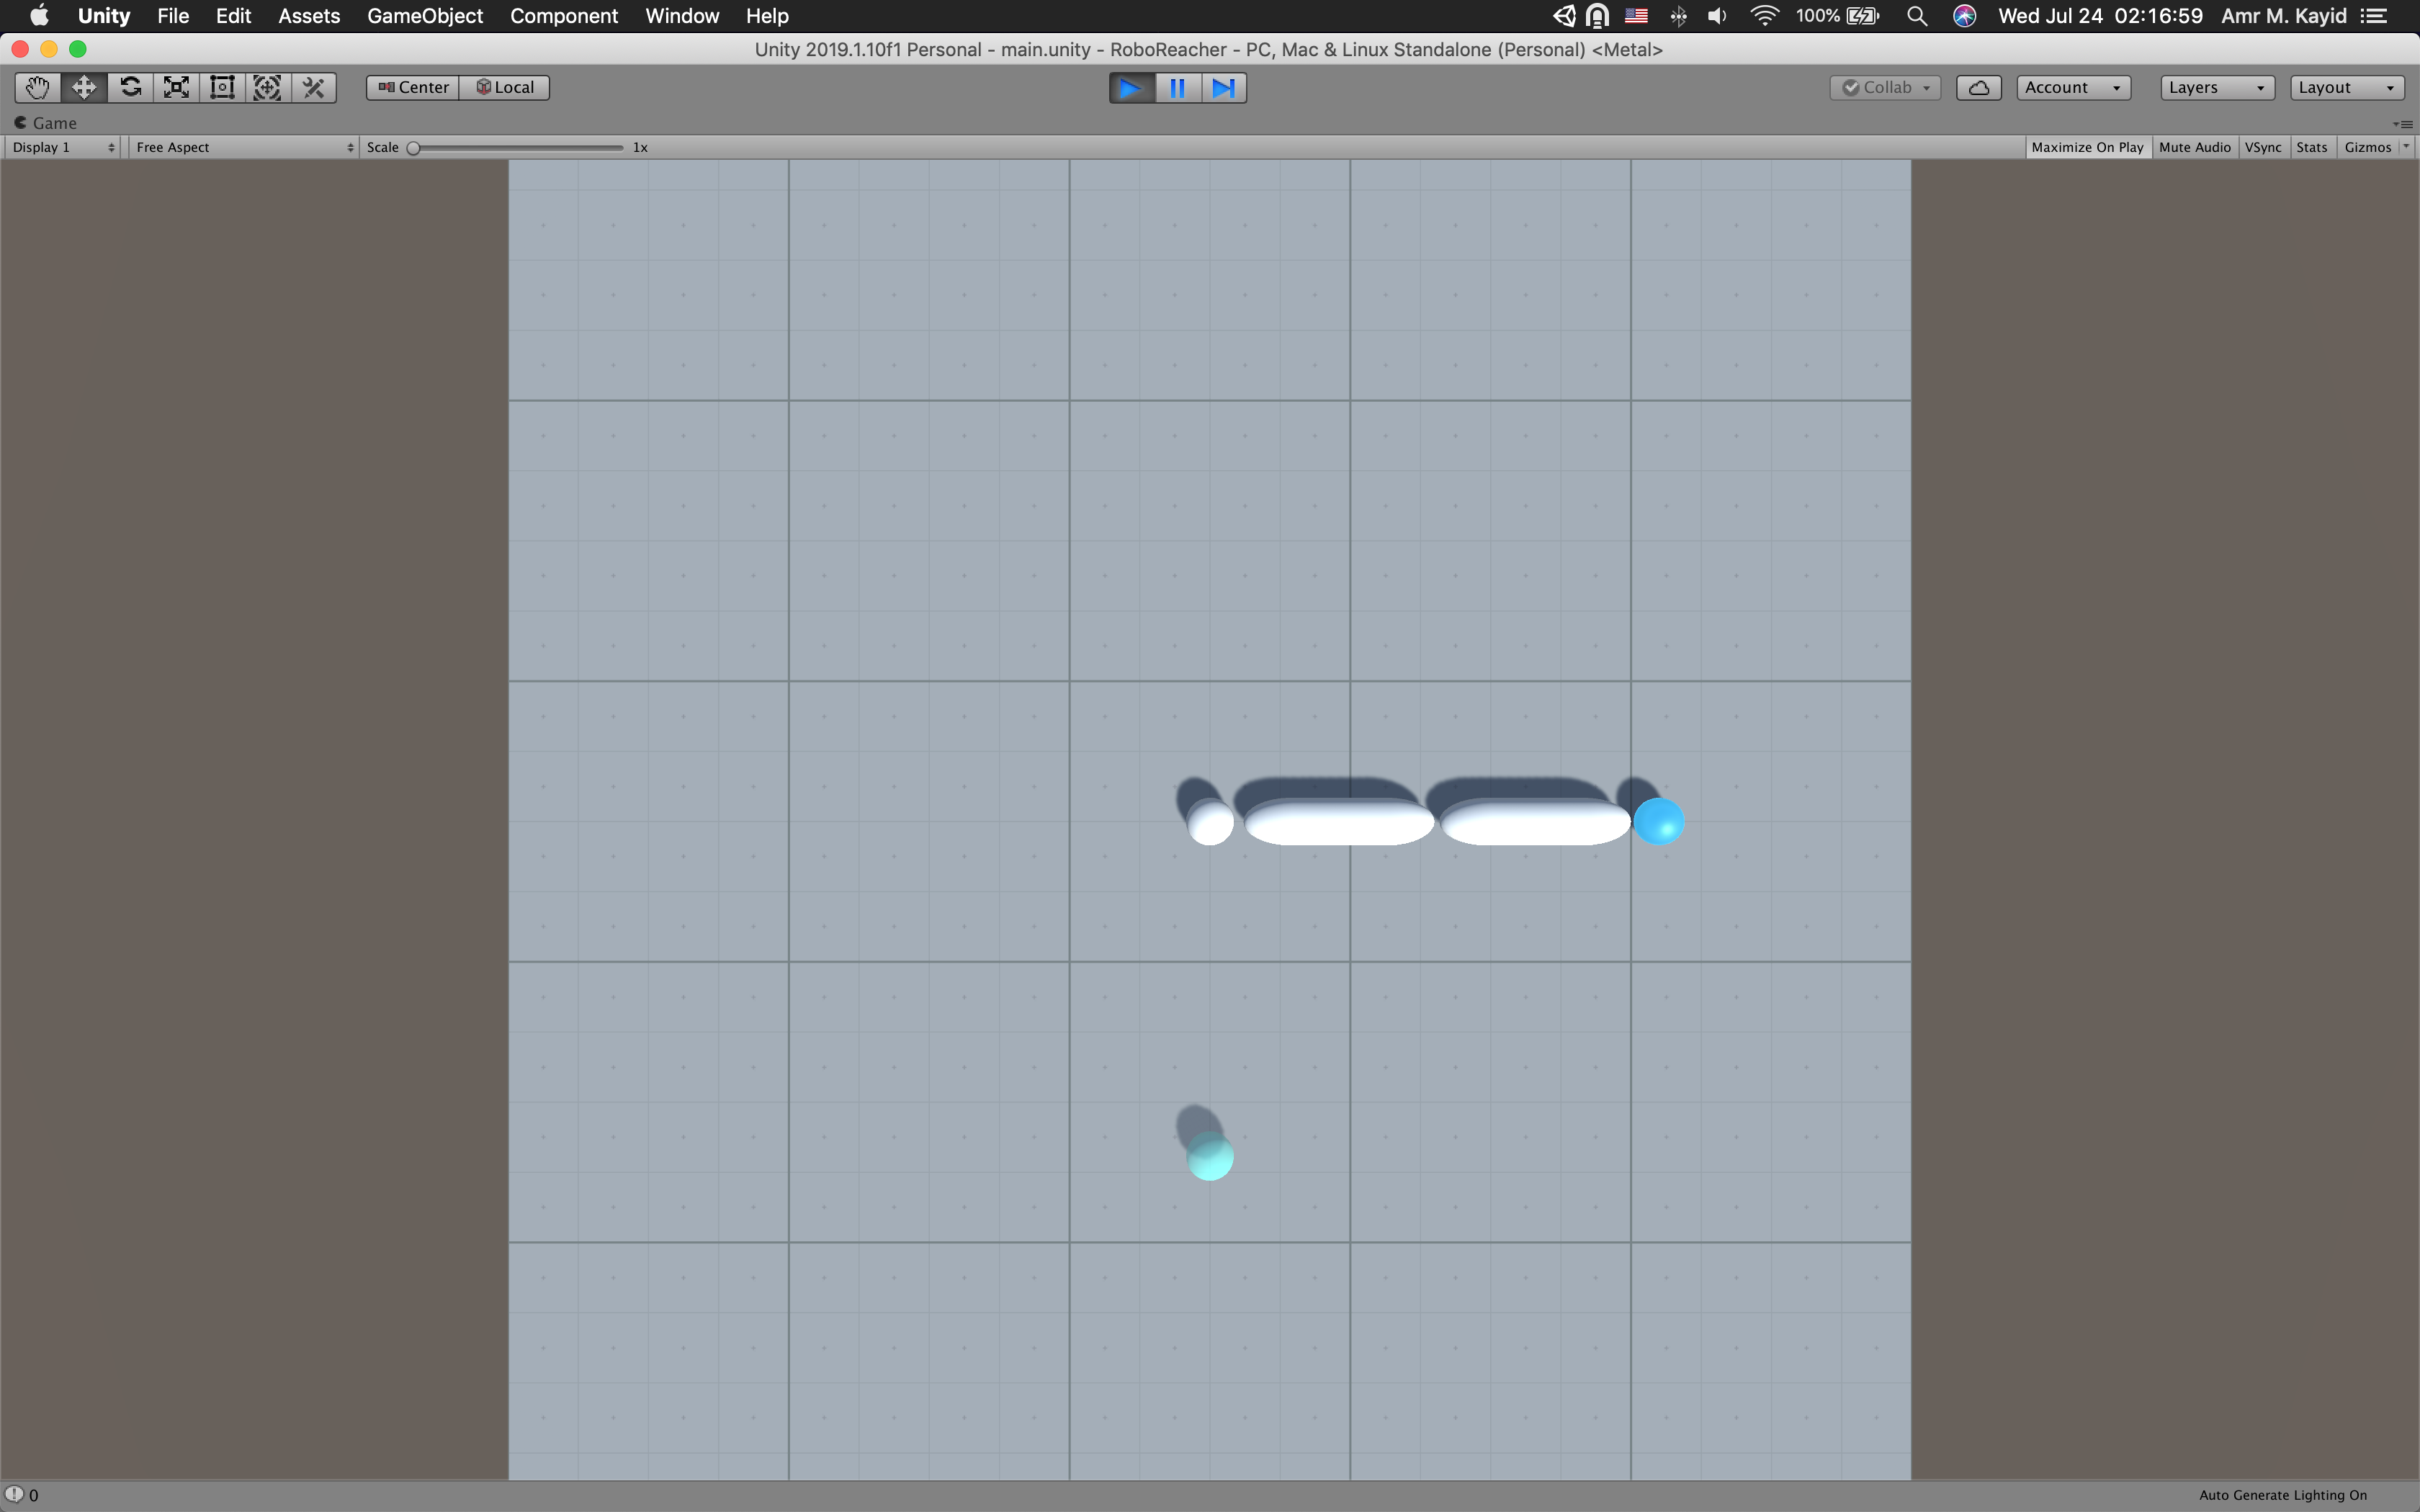
\includegraphics[width=0.7\linewidth]{figures/envs/unity_roboreacher.png}
				\caption{Unity 2-DOF Environment}
				\label{fig:unity_reacher}
\end{figure}

\subsubsection{Reward Function}

The reward function for this environment is different as we modify it to only give a reward of (+0.1) for the agent if the agent can reach the target sphere and keep moving with it along a circular path.


\subsubsection{Experiment Results}

Since this is an evaluation experiment where we have the trained agent from the 3rd experiment, the evaluation will be based on the average reward the agent can obtain after running for 1M time-steps. In this experiment, the agent was able to obtain an average reward ranging from 15 to 20 over the whole testing time-steps as shown in the figure below.

\begin{figure}[!htb]
		\centering
				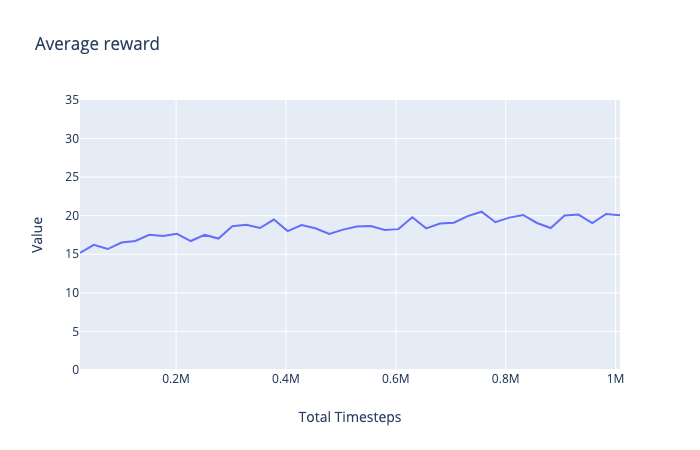
\includegraphics[width=\linewidth]{figures/exps/unity2d.png}
				\caption{Unity 2-DOF Average Reward}
				\label{fig:unity2d_avg_reward}
\end{figure}


\subsubsection{Conclusion}

In this experiment, we perform a training and evaluation for the simple robotic task using ppo algorithm in non-distributed setup to train our agent. we conclude that the experiment took a large amount of time to train the agent (4 hours) and at the end the agent didn't solve the required task and the learning process was not successful. 
\clearpage 